%%%%%%%%%%%%%%%%%%%%%%%%%%%%%%%%%%%%%%%%%%%%%%%%%%%%%%%%%%%%%%%%%%%%%%%%%%%%%%%%
%2345678901234567890123456789012345678901234567890123456789012345678901234567890
%        1         2         3         4         5         6         7         8

\documentclass[letterpaper, 10 pt, conference]{ieeeconf}

\IEEEoverridecommandlockouts
\overrideIEEEmargins

\usepackage{graphicx}
\usepackage{mathptmx}
\usepackage{times}
\usepackage{amsmath}
\usepackage{amssymb}
\usepackage{booktabs}
\usepackage{multirow}
\usepackage{siunitx}

\usepackage[style=ieee, url=false, doi=false, isbn=false, eprint=false]{biblatex}
\addbibresource{refs.bib}

\title{\LARGE \bf
Teleoperation for Bimanual Dexterous Manipulation \\ via Multi-Demonstration Residual Learning}

\author{Jeffrey Yu$^{1}$, Cheng Pan$^{1}$, and Josie Hughes$^{1}$% <-this % stops a space
\thanks{$^{1}$The authors are with the CREATE Lab, Swiss Federal Institute of Technology Lausanne (EPFL), 1015 Lausanne, Switzerland}%
}

\begin{document}

\maketitle
\thispagestyle{empty}
\pagestyle{empty}

%%%%%%%%%%%%%%%%%%%%%%%%%%%%%%%%%%%%%%%%%%%%%%%%%%%%%%%%%%%%%%%%%%%%%%%%%%%%%%%%
\begin{abstract}

Reinforcement learning guided by human demonstrations can produce high-fidelity
bimanual dexterous manipulation in simulation, but existing methods fit a separate
residual policy to each reference trajectory. Such a policy memorises one kinematic
path and is brittle when the input deviates from it, which is unavoidable under live
teleoperation. We train a single shared residual policy across a \emph{set} of
demonstrations that vary in starting configuration and approach direction, on top of a
frozen hand-motion imitator, so that the policy learns the manipulation skill rather
than a specific trajectory. To collect these demonstrations and to drive the
policy at run time we build a bimanual capture pipeline that fuses Apple Vision Pro
hand tracking with OptiTrack object poses through a cross-system Umeyama calibration
and streams them into Isaac Gym at \SI{60}{\hertz}. On two long-horizon bimanual tasks
--- capping an alcohol burner and flipping a brush --- the residual policy is the only
method evaluated that completes the full sequence offline, seating the cap in $7/10$
held-out demonstrations where an optimization-based retargeter seats it in $0/10$
despite transporting it perfectly. Under live teleoperation the same policy, without
retraining, completes the capping task on trajectories never seen during training.

\end{abstract}

%%%%%%%%%%%%%%%%%%%%%%%%%%%%%%%%%%%%%%%%%%%%%%%%%%%%%%%%%%%%%%%%%%%%%%%%%%%%%%%%
\section{Introduction}

Dexterous bimanual manipulation --- tasks requiring two hands to coordinate precisely
around a shared object --- remains one of the most challenging problems in robotics.
Contact-rich interactions demand not only accurate finger positioning but also the
ability to adapt forces and contacts in real time. Classical motion planning struggles
to scale to the dimensionality of two dexterous hands, while hand-coded controllers are
brittle to variation in object placement or operator intent.

Reinforcement learning (RL) offers a principled alternative, and human demonstrations
reduce the exploration burden by turning the problem into trajectory
tracking~\cite{maniptrans, dexmachina, dextrack}. Recent work shows that RL policies
guided by hand-object demonstrations achieve high-fidelity bimanual manipulation in
simulation~\cite{maniptrans}. For real-world deployment, however, the policy must
respond to \emph{live} human input rather than a fixed recording. At teleoperation time
the incoming motion inevitably differs from any trajectory seen during training: the
operator may approach from a different angle, use a different grasp, or vary timing.
The central challenge is therefore \emph{demonstration generalization} --- can a single
policy handle unseen trajectories of the same task?

Existing approaches address this only partially. ManipTrans~\cite{maniptrans} and
DexMachina~\cite{dexmachina} each fit a separate residual policy per demonstration, and
QuasiSim~\cite{quasisim} optimizes each trajectory independently at a cost of tens of
GPU-hours per sequence. A policy trained this way memorises the specific kinematic path
of that demonstration. DexTrack~\cite{dextrack} and Dexplore~\cite{dexplore} do train a
single controller across many references, but both are driven by recorded motion-capture
corpora rather than live operator input, and neither targets the bimanual residual
setting. This motivates a shift in training objective: instead of fitting one
demonstration, we train a single shared policy across a set of demonstrations that vary
in starting configuration, approach direction and grasp style.

Our contributions are twofold:

\begin{itemize}
\item \textbf{A bimanual teleoperation and data-collection pipeline} integrating the
Apple Vision Pro (AVP) and OptiTrack motion capture, with cross-system spatial
calibration via the Umeyama algorithm~\cite{umeyama}, recording synchronized hand and
object trajectories at \SI{60}{\hertz} and streaming them into Isaac Gym. The same
hardware path serves both capture and live teleoperation without modification.

\item \textbf{A single residual policy that generalizes across unseen demonstration
trajectories}, demonstrated on two long-horizon bimanual tasks. In contrast to prior
work~\cite{maniptrans}, which requires a policy per demonstration, ours is trained
jointly on demonstrations varying in starting configuration and grasp approach, and
teleoperates the task on trajectories not seen during training.
\end{itemize}

%%%%%%%%%%%%%%%%%%%%%%%%%%%%%%%%%%%%%%%%%%%%%%%%%%%%%%%%%%%%%%%%%%%%%%%%%%%%%%%%
\section{Related Work}

\subsection{Dexterous Manipulation via RL}

Large-scale RL with domain randomization enables in-hand cube
reorientation~\cite{openai_cube}, and DeXtreme extends this to hardware through
sim-to-real transfer~\cite{dextreme}. These learn from scratch with task-specific
rewards, which limits generalization to new tasks. Reference-guided RL reduces this
burden by supplying a demonstration as a tracking objective~\cite{deepmimic}. Applied to
dexterous hands, DexTrack trains a neural tracking controller from human
references~\cite{dextrack} and Dexplore uses reference-scoped
exploration~\cite{dexplore}. Dexplore argues that the staged decomposition ---
retargeting, tracking and residual correction --- leaves demonstrations underused and
compounds error across stages, replacing it with a single-loop optimization that treats
the demonstration as soft guidance. We retain the staged design for a different reason:
freezing the imitator yields a policy that runs against an arbitrary incoming target
stream at control rate, which is what makes live teleoperation possible, whereas an
optimization coupled to a demonstration corpus has no equivalent inference-time
counterpart. ManipTrans~\cite{maniptrans} introduces the two-stage framework we build
on, pre-training a generalist imitator on large-scale hand motion and fine-tuning a
residual per demonstration; DexMachina~\cite{dexmachina} similarly trains
per-demonstration policies. Both achieve strong performance on their training
demonstrations but do not generalize to unseen trajectories of the same task.

\subsection{Teleoperation and Retargeting}

DexPilot formulates vision-based dexterous teleoperation around task-space fingertip
objectives~\cite{dexpilot}, and AnyTeleop generalizes this across
embodiments~\cite{anyteleop}. OpenTeach~\cite{openteach} and
Bunny-VisionPro~\cite{bunnyvisionpro} demonstrate low-latency teleoperation with
consumer hand tracking, and Open-TeleVision~\cite{opentv} adds immersive visual
feedback. TeleDexter~\cite{teledexter}, evaluated on single-hand manipulation,
introduces the random action-masking augmentation we adopt. A common pattern across
these systems is direct joint retargeting: human joint angles are mapped to robot
targets via kinematic correspondences and streamed at control frequency, without a
learned policy that adapts to contact forces. Recent work incorporates contact geometry
into the retargeting objective itself~\cite{toporetarget}. In contrast, our approach
inserts a trained RL residual between operator commands and robot actions, supplying
the compliance and contact correction a retargeting-only pipeline cannot.

\subsection{Data Collection}

DexCap~\cite{dexcap} combines a wrist-mounted SLAM camera with OptiTrack markers;
OakInk-V2~\cite{oakinkv2} and ARCTIC~\cite{arctic} capture bimanual sequences with
optical motion capture. These pipelines recover hand parameters through offline
optimization-based retargeting after capture. The AVP instead provides
MANO-compatible~\cite{mano} keypoints directly at capture time, eliminating the
post-processing stage and allowing the same pipeline to drive live teleoperation.

%%%%%%%%%%%%%%%%%%%%%%%%%%%%%%%%%%%%%%%%%%%%%%%%%%%%%%%%%%%%%%%%%%%%%%%%%%%%%%%%
\section{Method}

\subsection{Problem Formulation}

A pair of robotic hands $\mathbf{d} = \{d_l, d_r\}$ must reproduce a manipulation
demonstrated by human hands $\mathbf{h} = \{h_l, h_r\}$ interacting with objects
$\mathbf{o} = \{o_l, o_r\}$. A demonstration provides a hand trajectory
$\mathcal{T}^h = \{\tau^t_h\}_{t=1}^{T}$ encoding wrist 6-DoF pose, linear and angular
velocity and finger joint positions, and an object trajectory
$\mathcal{T}^o = \{\tau^t_o\}_{t=1}^{T}$. All translations are expressed relative to the
wrist to reduce spatial complexity while preserving the direction of gravity. We model
the task as an MDP; the action for each hand comprises target joint positions
$a^t_q \in \mathbb{R}^K$ for PD control of the fingers and a 6-DoF wrench
$a^t_w \in \mathbb{R}^6$ applied to the wrist.

\subsection{Two-Stage Policy Architecture}

We adopt the two-stage decomposition of ManipTrans~\cite{maniptrans}
(Fig.~\ref{fig:architecture}). The difference lies in how we use it: instead of fitting
a separate policy to each individual demonstration, we train a single shared policy
across a set of demonstrations.

\textbf{Stage 1 --- imitator.} The imitator $\pi_I$ is a pre-trained generalist policy
driving each hand to track the reference trajectory without object interaction. Its
state is $s^t_I = \{\tau^t_h, s^t_\mathrm{prop}\}$, where
$s^t_\mathrm{prop} = \{q^t_d, \dot{q}^t_d, w^t_d, \dot{w}^t_d\}$ are the finger joint
angles and wrist pose with their velocities. We use the imitator released with
ManipTrans directly and do not retrain it.

\textbf{Stage 2 --- residual.} A residual module $\pi_R$ refines the imitator output to
satisfy the physical constraints of object interaction. Its state
$s^t_R = s^t_I \cup s^t_\mathrm{interact}$ augments the imitation state with
\begin{equation}
    s^t_\mathrm{interact} = \bigl\{
        \tau^t_o,\; p^t_{\hat{o}},\; \dot{p}^t_{\hat{o}},\;
        m_{\hat{o}},\; G_{\hat{o}},\; \mathrm{BPS}(\hat{o}),\;
        D(j^t_d, p^t_{\hat{o}}),\; C^t
    \bigr\},
\end{equation}
where $p^t_{\hat{o}}$ and $\dot{p}^t_{\hat{o}}$ are the simulated object position
(wrist frame) and velocity, $m_{\hat{o}}$ and $G_{\hat{o}}$ its centre of mass and
gravitational force, $\mathrm{BPS}(\hat{o})$ a Basis Point Set encoding~\cite{bps} of
the shape, $D(\cdot)$ the squared distance from each hand keypoint to the object, and
$C^t$ the per-fingertip contact force from the simulator. The correction
$\Delta a^t_R \sim \pi_R(\Delta a^t \mid s^t_R, a^t_I, a^{t-1})$ is added element-wise,
$a^t = a^t_I + \Delta a^t_R$, clipped to joint limits. Following~\cite{maniptrans} the
residual is initialized with a zero-mean Gaussian and warmed up linearly, which prevents
collapse. During training the imitator weights are frozen; only the residual is updated.

\begin{figure}[tb]
     \centering
     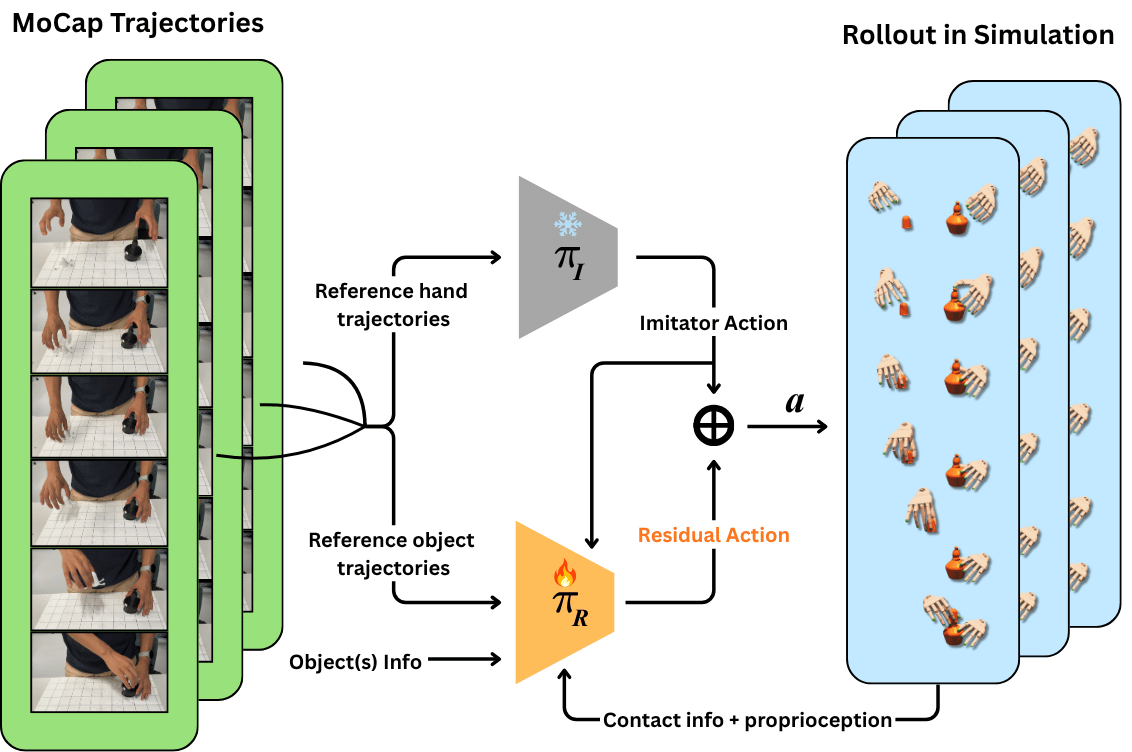
\includegraphics[width=\columnwidth]{Figs/multimaniptransarchitecture.png}
     \caption{System architecture. A hand-motion imitation model pre-trained on
     large-scale human demonstrations is frozen, and a residual policy is trained on top
     of it across a set of demonstrations rather than a single reference.}
     \label{fig:architecture}
\end{figure}

\subsection{Reward}

The imitator reward combines wrist tracking, finger keypoint tracking and smoothness,
$r^t_I = w_\mathrm{wrist} r^t_\mathrm{wrist} + w_\mathrm{finger} r^t_\mathrm{finger} +
w_\mathrm{smooth} r^t_\mathrm{smooth}$, with the finger term
$r^t_\mathrm{finger} = \sum_{f=1}^{F} w_f \exp(-\lambda_f \|j^t_{d_f} - j^t_{h_f}\|_2^2)$
over $F = 21$ MANO-corresponding keypoints~\cite{mano}, weighted towards the thumb,
index and middle fingertips. For the residual stage we add two object-centric terms,
\begin{equation}
    r^t_R = r^t_I + w_\mathrm{object} r^t_\mathrm{object} +
    w_\mathrm{contact} r^t_\mathrm{contact},
\end{equation}
where $r^t_\mathrm{object}$ penalizes positional and velocity deviation of the simulated
object from its reference, and $r^t_\mathrm{contact}$ rewards fingertip force whenever
the reference hand-to-object distance falls inside a contact band (linearly ramped
between \SI{3}{\centi\meter} and \SI{2}{\centi\meter}). The formulation deliberately
avoids task-specific engineering, keeping the signal general across demonstrations.

\subsection{Demonstration Augmentation}

To expose one policy to a distribution of trajectories rather than a single path, each
demonstration is augmented at load time. All spatial augmentations spin the scene about
a vertical axis, so objects stay upright on the table: $p_t \mapsto R(p_t - c_t) + c_t$
with $R = R_z(\theta)$ about a per-frame pivot $c_t$, with the matching velocity
correction. The variants differ in which bodies move and what serves as the pivot ---
rotating the right hand about the left hand's object (the only augmentation that varies
\emph{inter-hand} geometry, drawn per demonstration by rejection sampling so the start
position shifts by at most \SI{5}{\centi\meter}), orbiting a hand about the object it
already holds, and rotating an object's orientation while the hand stays fixed, which
deliberately breaks the demonstrated grasp alignment. Additive keypoint noise drawn from
$\mathcal{U}(-\sigma, +\sigma)$ with $\sigma = \SI{0.5}{\centi\meter}$ emulates
estimator error. Finally, following TeleDexter~\cite{teledexter}, a random subset of
joints is periodically frozen at its previously commanded target so the policy cannot
assume every degree of freedom responds on schedule; the maximum freeze duration is
annealed over training.

%%%%%%%%%%%%%%%%%%%%%%%%%%%%%%%%%%%%%%%%%%%%%%%%%%%%%%%%%%%%%%%%%%%%%%%%%%%%%%%%
\section{Experimental Setup}

\subsection{Capture and Teleoperation Pipeline}

Data collection and teleoperation use the same two systems (Fig.~\ref{fig:pipeline}).
Using the AVP SDK and VisionProTeleop~\cite{visionproteleop} we collect 21 keypoints and
the wrist pose per hand; OptiTrack records the object poses. The objects for the capping
task are an alcohol burner and its cap, sourced from OakInk2~\cite{oakinkv2} mesh files
and modified to carry OptiTrack markers; the brush task uses a
$2.5 \times 20 \times 1.5$\,cm prism sized after a toothbrush and a
$4 \times 5 \times 4$\,cm cup. Markers were placed so as to minimally affect the
operator's manipulation.

Because the two systems have independent coordinate frames, we calibrate with a tracker
on the right index fingertip, moving the hand through the shared workspace and solving
for the rigid map with the Umeyama algorithm~\cite{umeyama}. The mapping is imperfect,
attributable to the image-based estimation the AVP uses for finger and wrist pose and to
tracker placement varying slightly between sessions; remapping error correlates
positively with hand speed. At a reasonable manipulation speed of
\SIrange{200}{400}{\milli\meter\per\second} the RMSE between systems is
\SIrange{8}{12}{\milli\meter}.

At run time the laptop fuses both streams into a common frame, stamps each frame with a
sequence number and capture time, and publishes it as \texttt{msgpack} over a ZeroMQ
\textsc{pub} socket at \SI{60}{\hertz}. The desktop subscribes and steps the policy in
Isaac Gym~\cite{isaacgym} at roughly \SI{60}{\hertz}. Because the consumer runs below
the publisher rate, the transport delivers the newest frame and discards the backlog
rather than queueing it; a FIFO would let latency accumulate without bound across a
session. The rendered viewer returns to the laptop over VNC at \SI{15}{\hertz}, closing
the loop for the operator.

\begin{figure}[tb]
     \centering
     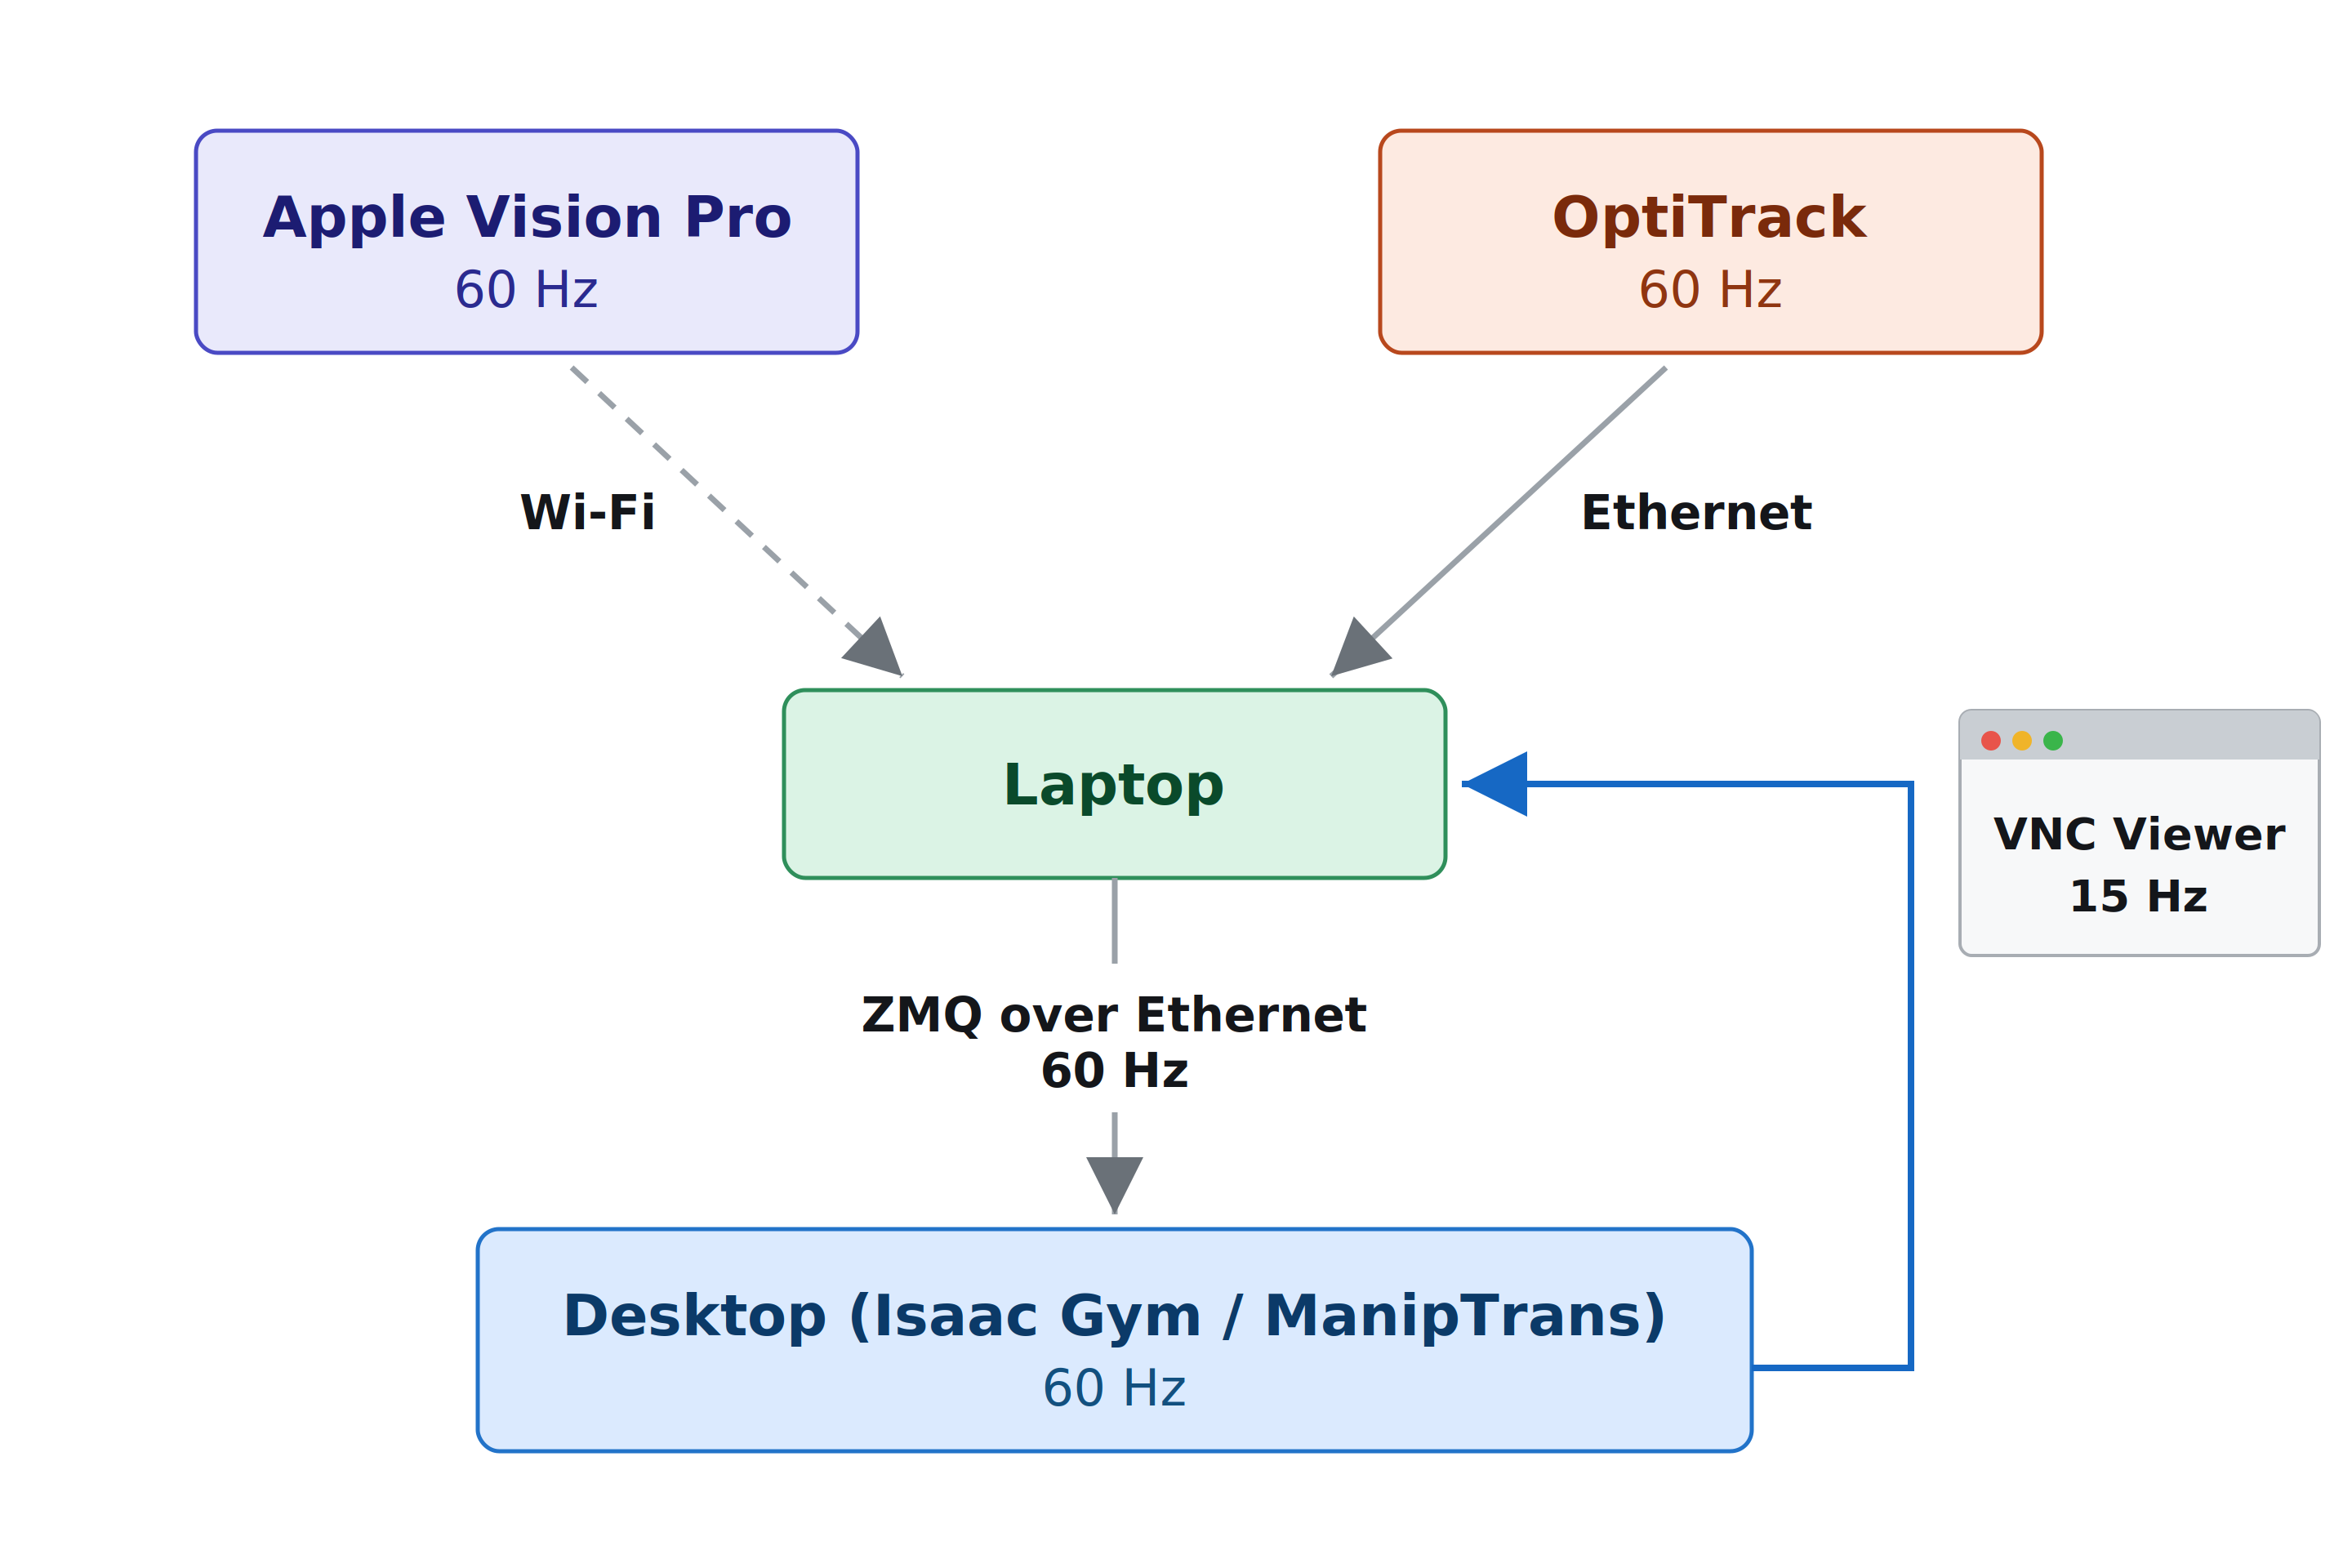
\includegraphics[width=\columnwidth]{Figs/data_collection_pipeline_zmq_v11.png}
     \caption{Live capture and teleoperation pipeline. Annotated values are the measured
     rate of each stage in \si{\hertz}.}
     \label{fig:pipeline}
\end{figure}

\subsection{Tasks and Demonstrations}

Both tasks embody real-world scenarios (Fig.~\ref{fig:tasks}). In \textbf{bottle
capping}, the left hand stabilizes a laboratory alcohol burner while the right hand
picks up the cap and seats it; demonstrations are collected from five reach distances,
spaced approximately \SI{5}{\centi\meter} apart, with deliberately scattered approach
angles at each distance. In \textbf{brush flipping}, the left hand grasps the brush end
and lifts it, the right hand grasps the bristled end, both hands rotate the brush about
its centre, the left hand releases, and the right hand places it back into the cup ---
a longer-horizon task with a bimanual handover. Here the brush starts at a fixed
orientation and the trajectory is varied instead by lifting it to different heights and
rotating it at different speeds.

\begin{figure*}[tb]
     \centering
     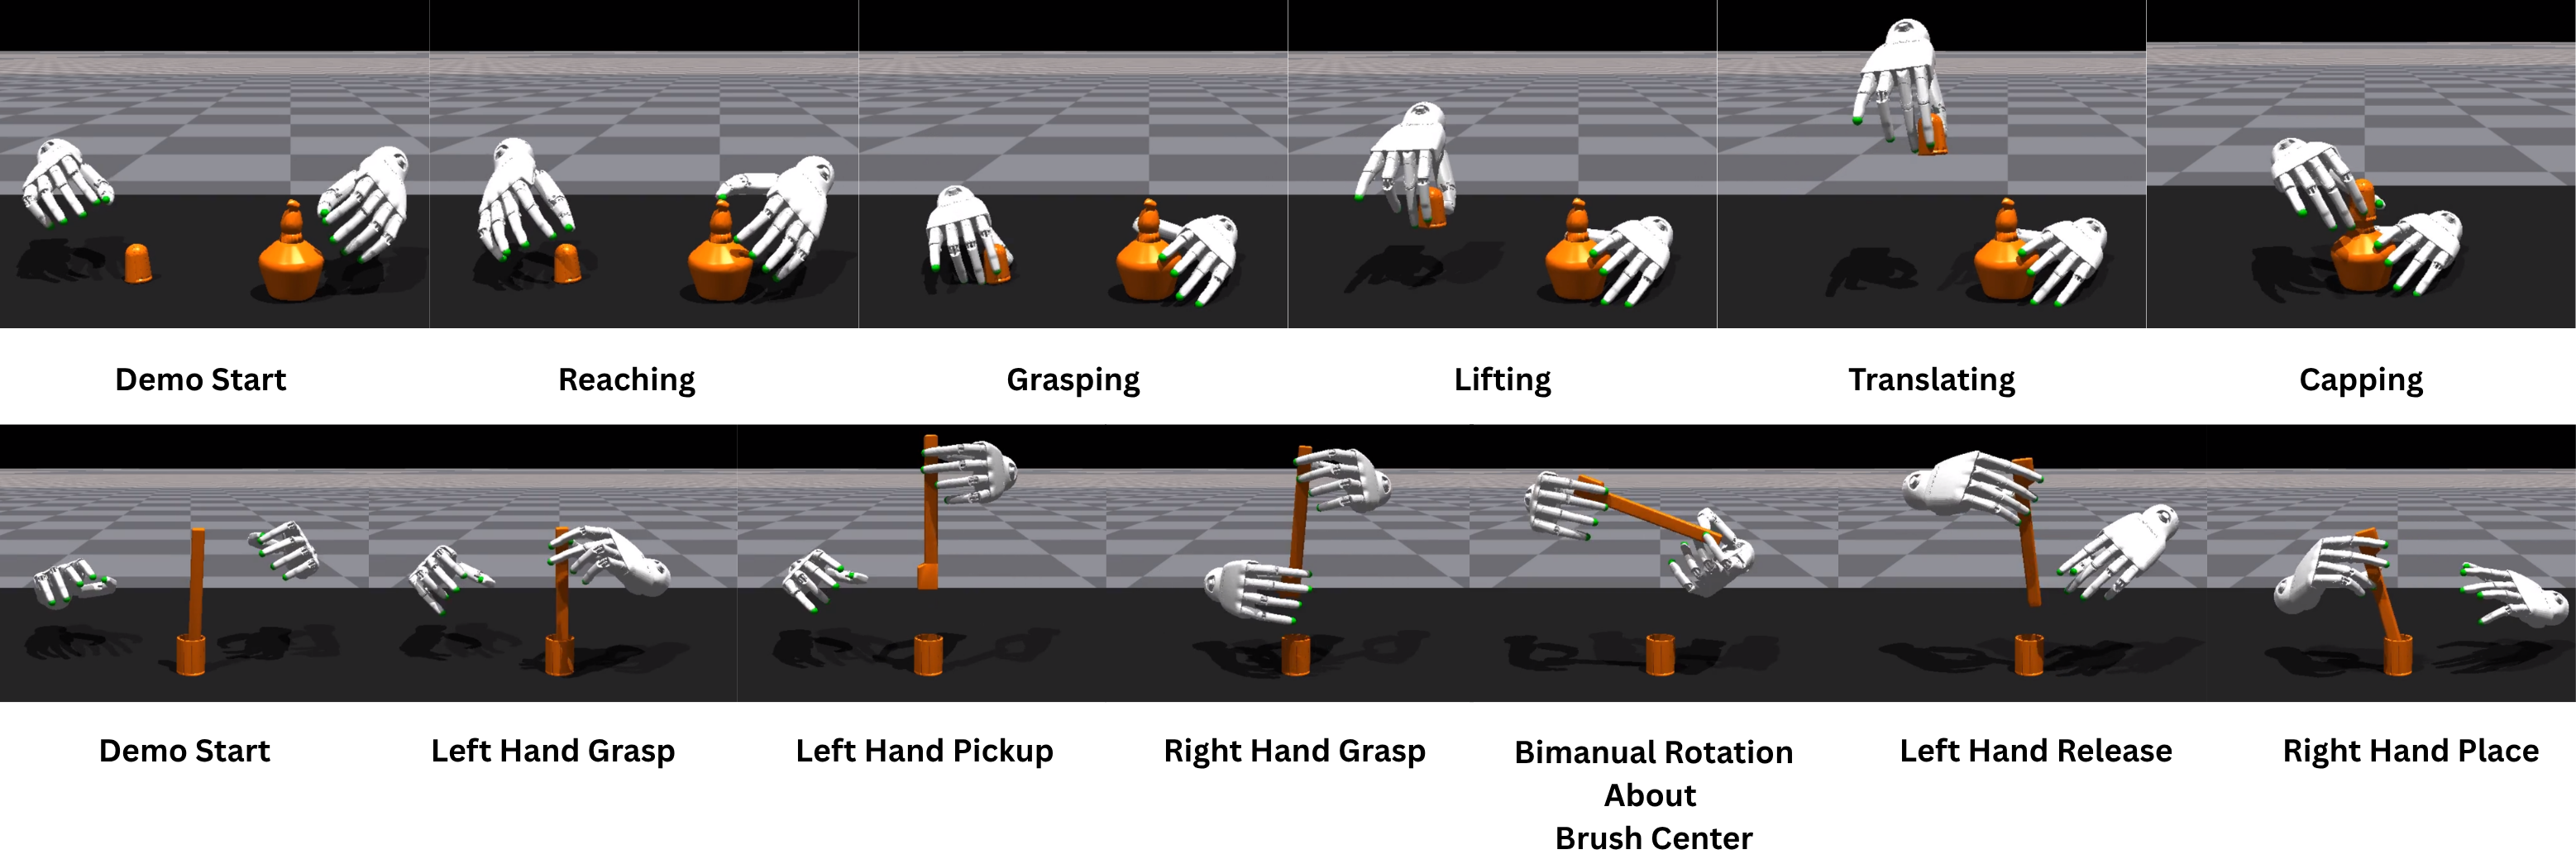
\includegraphics[width=0.92\textwidth]{Figs/brush_bottle_task_breakdown.png}
     \caption{Task decomposition of the bottle-capping (top) and brush-flipping (bottom)
     manipulation tasks. Each phase is scored independently in
     Tables~\ref{tab:offline}--\ref{tab:teleop}.}
     \label{fig:tasks}
\end{figure*}

\subsection{Baselines and Metrics}

We compare the full residual-imitation model against dex-retargeting~\cite{anyteleop},
a classical optimization-based method, and against the frozen pre-trained imitator
alone. The residual is trained with PPO~\cite{ppo} optimized by Adam~\cite{adam} in
Isaac Gym~\cite{isaacgym}, on an HPC cluster with V100 and A100 GPUs; evaluation and
teleoperation run on a single RTX 4090.

For offline rollouts we use three metrics following~\cite{maniptrans}, averaged over
successful rollouts with bimanual metrics computed per hand: object translation error
$E_t$, object rotation error $E_r$, and mean per-fingertip error $E_{ft}$ over the
index and thumb, the two digits that dominate these tasks. A rollout succeeds if
$E_r < 45^\circ$, $E_t < \SI{3}{\centi\meter}$ and $E_{ft} < \SI{6}{\centi\meter}$, with
both hands satisfying all conditions simultaneously. Because $E_{ft}$ is restricted to
two fingertips rather than the full set, success rates are not directly comparable with
those reported in~\cite{maniptrans}. We roll out each demonstration 128 times and report
the fraction that succeed. Online, task success is assessed qualitatively by visual
inspection, decomposed by phase.

For generalization we partition the 50 reach demonstrations --- 10 at each of five
distances --- into five folds by a deterministic stratified split, dealing two per
distance to each fold, so every fold holds out 10 demonstrations spanning all distances
and trains on the remaining 40. Throughout, \emph{zero-shot} denotes demonstrations held
out from the policy's training set.

%%%%%%%%%%%%%%%%%%%%%%%%%%%%%%%%%%%%%%%%%%%%%%%%%%%%%%%%%%%%%%%%%%%%%%%%%%%%%%%%
\section{Results}

\subsection{Offline Evaluation}

Table~\ref{tab:offline} separates the three methods by phase. All three complete the
approach identically --- 10/10 on reaching and stabilizing --- so the comparison is
decided in the contact phases.

The imitator fails at the first of them, grasping the cap in none of the 10
demonstrations. This is expected: it tracks the kinematic reference but has no mechanism
to respond to contact forces. When the hand closes, the fingers reach the reference
joint angles but without contact-aware correction the fingertips cannot generate
sufficient grip force to lift the cap. On the brush, the same failure mode is consistent
across all trials --- the fingertips approach but do not close around it, and the policy
proceeds open-loop as if the object were held.

The residual policy recovers this gap by conditioning on fingertip contact forces and
hand-to-object distances: all 10 demonstrations grasp the cap and 8/10 lift and
translate it, with 7/10 seating. On the brush it completes the full sequence in 5/10,
with failures distributed across the later phases rather than concentrated at the grasp;
the dominant mechanism is the handover, where the left hand fails to release cleanly
after the bimanual rotation.

The dex-retargeting baseline outperforms the residual policy over the transport phases,
matching it at the grasp (10/10) and exceeding it at lifting and translating (10/10
against 8/10). Solving directly for a fingertip configuration matching the operator's
hand geometry produces a repeatable, geometrically precise pinch. What it does not
control is the pose of the cap \emph{within} that pinch: without observation of
fingertip contact, the thumb and index do not close simultaneously, and whichever
contacts first rotates the cap between the fingertips before the grip settles. The pinch
is stable --- hence the 10/10 transport --- but stable about an orientation that differs
from the one at which the cap was grasped. Nothing downstream corrects this, so the cap
arrives at the bottle at an uncontrolled angle, and seating, which requires the cap axis
to align with the opening within a small tolerance, succeeds in none of the 10
demonstrations. On the brush the same limitation appears earlier: the vector-based
objective optimizes a different quantity than fingertip alignment, so the left hand
collides with or misses the brush rather than closing around it, and the method does not
progress beyond the initial reach.

\begin{table}[tb]
    \centering
    \caption{Phase-level success counts over 10 zero-shot demonstrations, offline.}
    \label{tab:offline}
    \begin{tabular}{llccc}
        \toprule
        \textbf{Task} & \textbf{Phase} & \textbf{dex-ret.} & \textbf{Imitator} & \textbf{Ours} \\
        \midrule
        \multirow{5}{*}{Capping}
            & Reach cap          & 10 / 10 & 10 / 10 & 10 / 10 \\
            & Grasp cap          & 10 / 10 &  0 / 10 & 10 / 10 \\
            & Lift cap           & 10 / 10 &  0 / 10 &  8 / 10 \\
            & Translate cap      & 10 / 10 &  0 / 10 &  8 / 10 \\
            & Seat cap           &  0 / 10 &  0 / 10 &  \textbf{7 / 10} \\
        \midrule
        \multirow{5}{*}{Brush}
            & Lift (L)           &  0 / 10 &  0 / 10 &  9 / 10 \\
            & Reach (R)          &  0 / 10 &  0 / 10 &  8 / 10 \\
            & Rotation (Bi)      &  0 / 10 &  0 / 10 &  8 / 10 \\
            & Release (L)        &  0 / 10 &  0 / 10 &  6 / 10 \\
            & Seat (R)           &  0 / 10 &  0 / 10 &  \textbf{5 / 10} \\
        \bottomrule
    \end{tabular}
\end{table}

\subsection{Generalization Across Demonstrations}

Fig.~\ref{fig:kfold} reports the five-fold cross-validation. Held-out success varies
substantially across folds and reach distances, with a mean of $0.56$. Low-scoring
demonstrations typically fail at the initial grasp, or form a grasp unstable enough that
the cap slips from between the fingertips. Performance broadly improves as reach
distance decreases, which we attribute to the hands being closer to the AVP and thus
more accurately tracked. Because each fold averages only 10 demonstrations, one or two
unusually hard demonstrations are enough to swing a fold mean, so individual fold
numbers should not be read as evidence on their own.

\begin{figure}[tb]
     \centering
     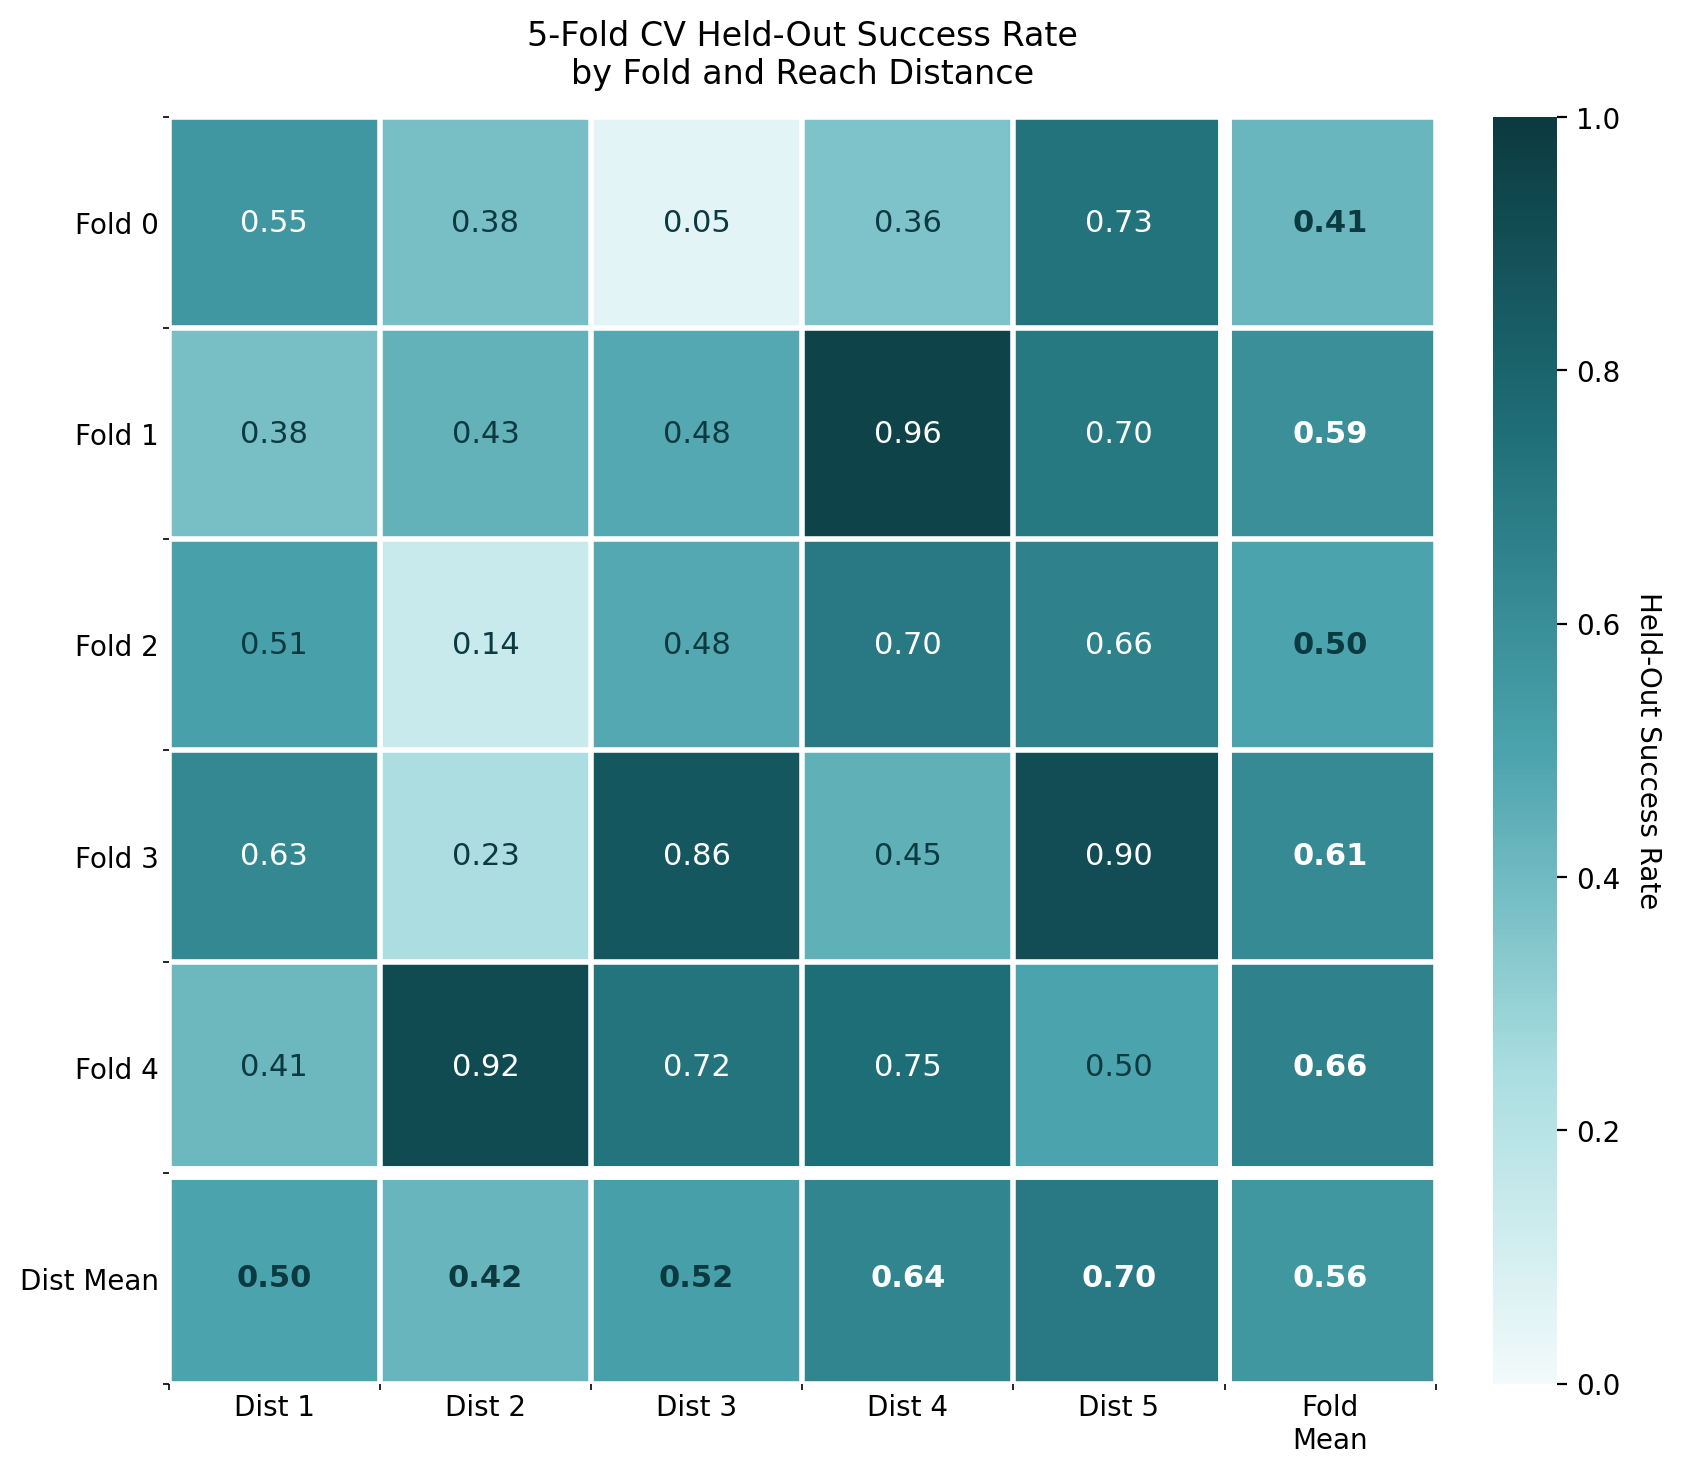
\includegraphics[width=0.92\columnwidth]{Figs/kfold_confusion_matrix_v2.png}
     \caption{Five-fold cross-validation held-out success rate by fold and reach
     distance. Each cell averages the two demonstrations in that (fold, distance) pair.}
     \label{fig:kfold}
\end{figure}

\begin{figure*}[!t]
     \centering
     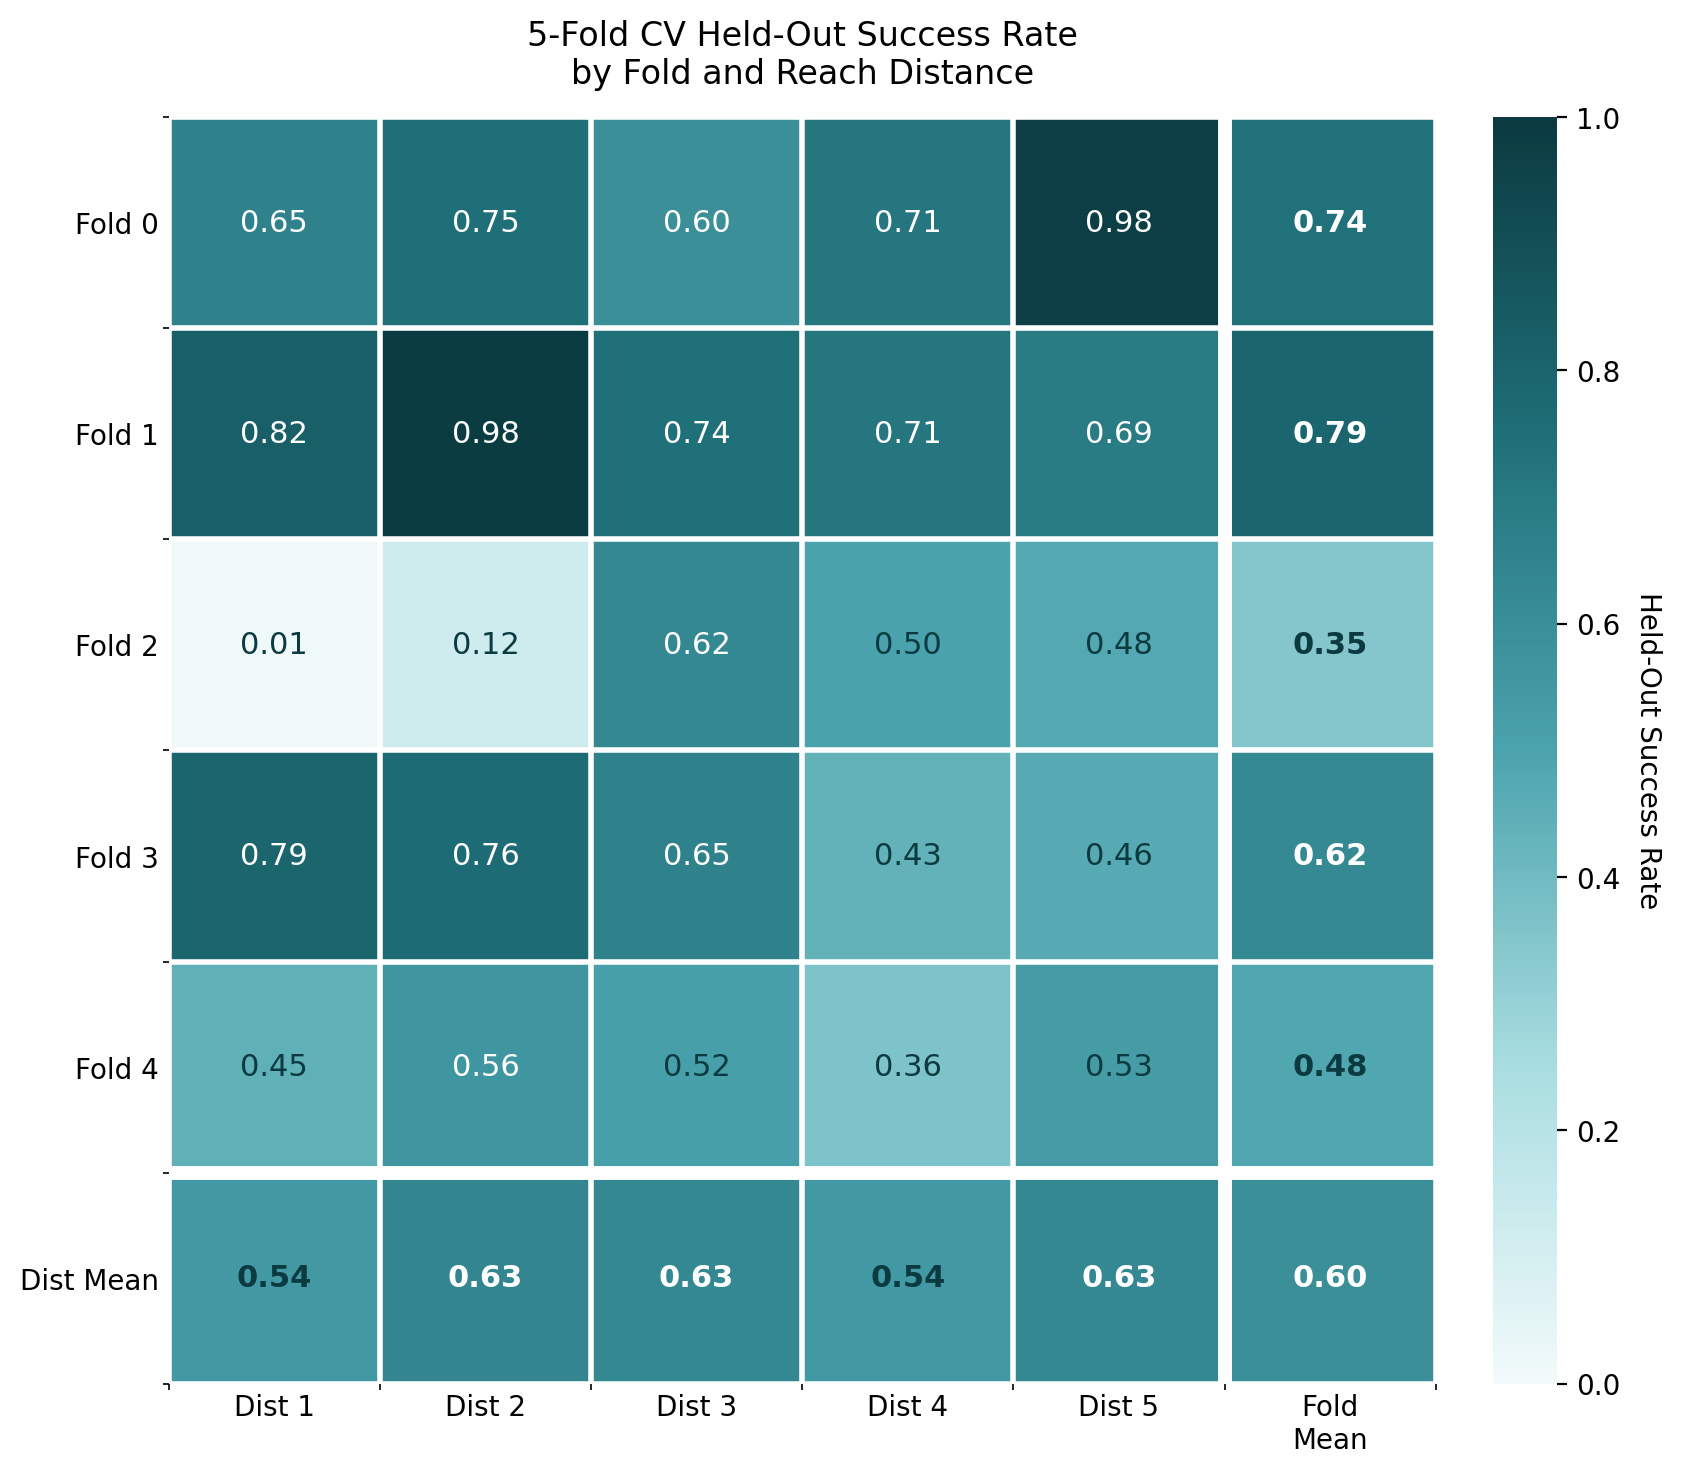
\includegraphics[width=0.42\textwidth]{Figs/kfold_confusion_matrix_objyaw_r2.png}
     \hspace{0.03\textwidth}
     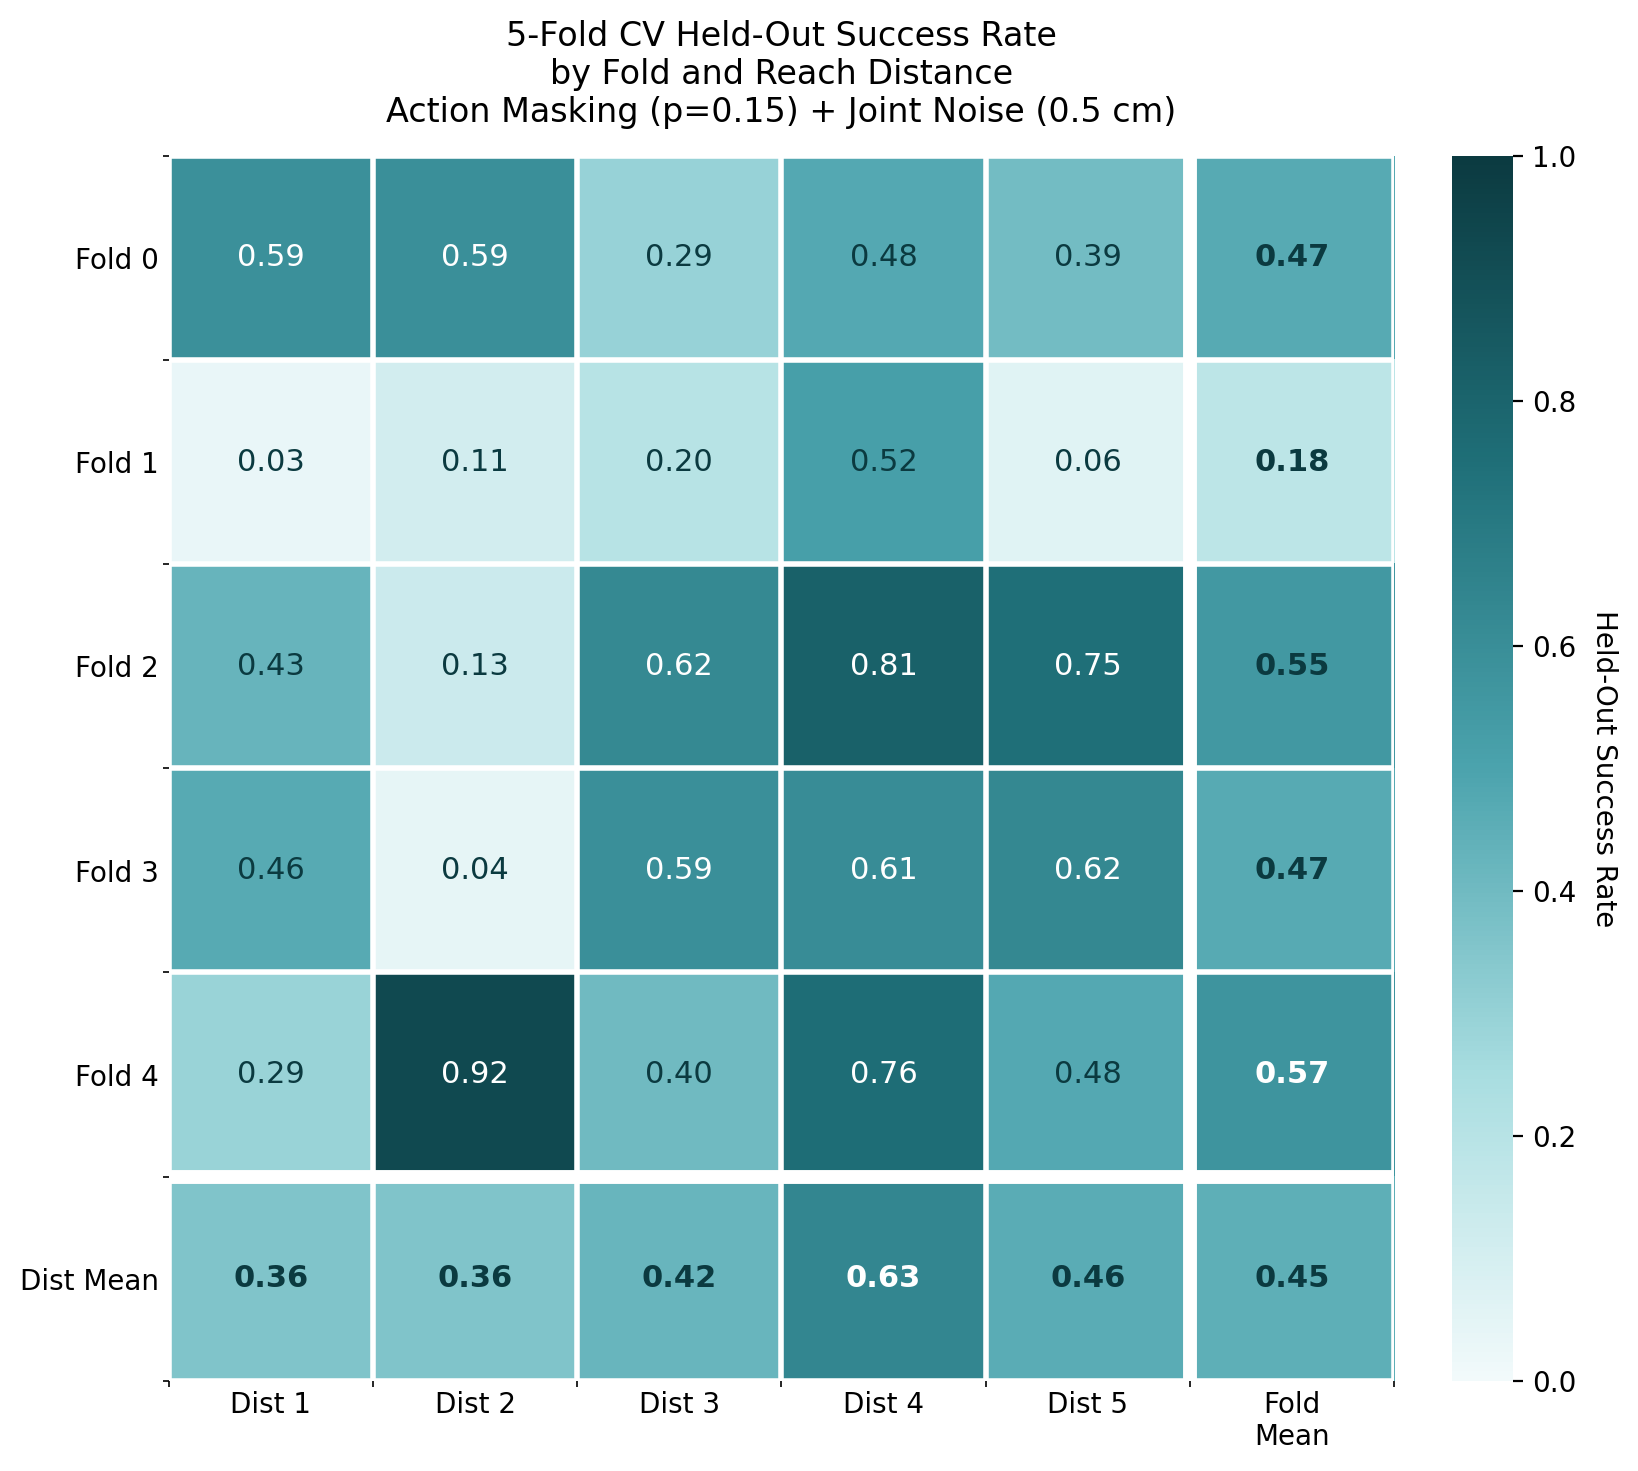
\includegraphics[width=0.42\textwidth]{Figs/kfold_confusion_matrix_v2_actmask_jn05.png}
     \caption{Augmentation ablation under the same five-fold protocol as
     Fig.~\ref{fig:kfold}. Left: object-yaw augmentation enabled (mean $0.60$), which
     flattens the distance marginals to $0.54$--$0.63$. Right: action masking and
     keypoint noise with object yaw disabled (mean $0.45$), where the distance
     dependence of the unaugmented baseline is unchanged.}
     \label{fig:augablation}
\end{figure*}

\subsection{Teleoperation}

Table~\ref{tab:teleop} reports 10 consecutive live trials per task. Qualitatively, the
residual model requires the least operator compensation: the grasping and capping
phases, the most interaction-heavy parts of the trajectory, are assisted by the policy.
It is nonetheless the only method to seat the cap at all (5/10), and completes the brush
rotation in 4/10, though no method seats the brush.

Dex-retargeting is the second most difficult to operate. The cap frequently rotates
during the pinch because the timing at which each fingertip contacts the surface is
determined entirely by the operator's motion; if index and thumb do not close at the
same rate, the asymmetric force tilts the cap rather than gripping it stably. This
forces the operator to compensate by rotating the entire wrist, making seating nearly
impossible. A three-finger grasp did not help: adding a third finger raises the number
of pairwise contact-timing differences from one to three, making synchronized contact
harder still. Pure kinematic retargeting therefore places the full burden of contact
coordination on the operator rather than the policy.

The imitation-only model is weakest: although the fingers close around the cap in all
ten trials, the grasp is secure enough to lift it in only one. Its coarse positional
targets bring the fingers into the vicinity of the cap but not precisely enough to seat
the fingertips on its surface with enough force to retain it, so the cap slips as the
hand lifts.

\begin{table}[tb]
    \centering
    \caption{Phase-level success counts over 10 consecutive teleoperation trials.}
    \label{tab:teleop}
    \begin{tabular}{llccc}
        \toprule
        \textbf{Task} & \textbf{Phase} & \textbf{dex-ret.} & \textbf{Imitator} & \textbf{Ours} \\
        \midrule
        \multirow{4}{*}{Capping}
            & Grasp cap          &  7 / 10 & 10 / 10 &  9 / 10 \\
            & Lift cap           &  7 / 10 &  1 / 10 &  9 / 10 \\
            & Translate cap      &  6 / 10 &  0 / 10 &  8 / 10 \\
            & Seat cap           &  0 / 10 &  0 / 10 &  \textbf{5 / 10} \\
        \midrule
        \multirow{4}{*}{Brush}
            & Lift (L)           &  7 / 10 &  0 / 10 & 10 / 10 \\
            & Reach (R)          &  5 / 10 &  0 / 10 &  9 / 10 \\
            & Rotation (Bi)      &  0 / 10 &  0 / 10 &  \textbf{4 / 10} \\
            & Seat (R)           &  0 / 10 &  0 / 10 &  0 / 10 \\
        \bottomrule
    \end{tabular}
\end{table}

Two qualitative failure modes recur, both consistent with distribution shift. First,
when the operator deliberately slows or pauses --- for instance while visually
cross-referencing the simulated hand against the real one --- the frame-to-frame deltas
fall outside the velocity distribution the policy was trained on. Second, the policy
becomes less stable during the capping phase at the end of the episode: as the two hands
converge on the burner they increasingly occlude one another and the object, degrading
the headset's keypoint estimates at precisely the moment the tracking targets must be
most accurate.

\subsection{Ablations}

\begin{figure}[tb]
     \centering
     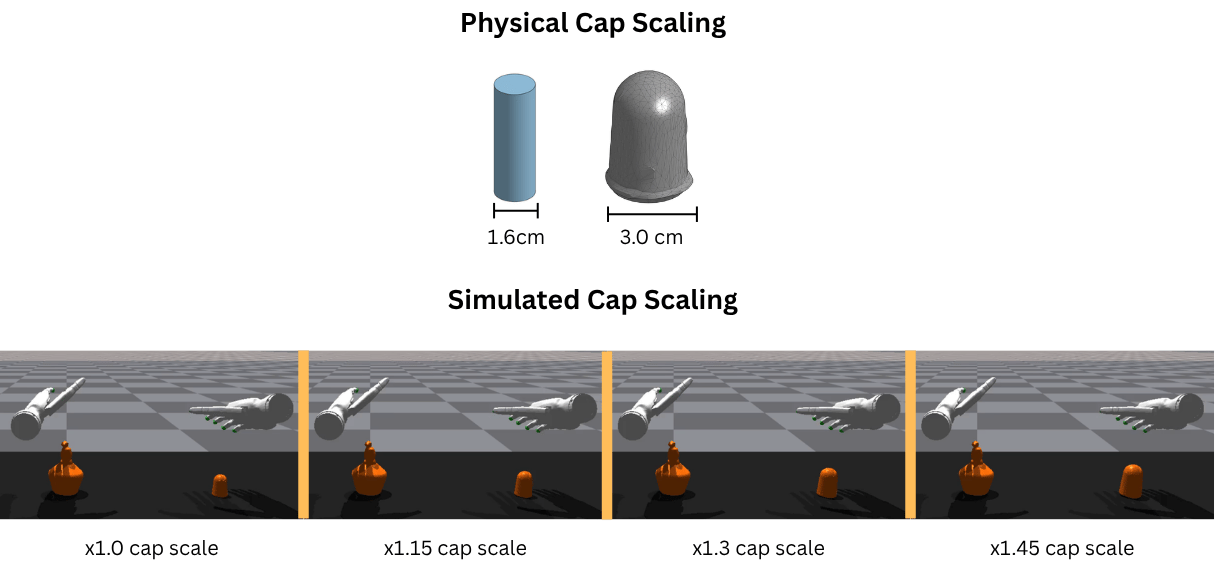
\includegraphics[width=\columnwidth]{Figs/physical_simulated_cap_scaling.png}
     \caption{Physical cap ablation (outer diameter reduced by \SI{1.4}{\centi\meter})
     and simulated ablation by scaling the mesh.}
     \label{fig:capscaling}
\end{figure}

\begin{table}[tb]
    \centering
    \footnotesize
    \caption{Cap-scaling ablation on the thin \SI{1.6}{\centi\meter} cap, successes out
    of 13. Reach omitted ($13/13$ throughout).}
    \label{tab:capablation}
    \begin{tabular}{llcccc}
        \toprule
        \textbf{Method} & \textbf{Phase} & $\times$\textbf{1.00} & $\times$\textbf{1.15}
        & $\times$\textbf{1.30} & $\times$\textbf{1.45} \\
        \midrule
        \multirow{4}{*}{dex-ret.}
            & Grasp     & 11 & 12 & 13 & 12 \\
            & Lift      & 10 & 12 & 13 & 11 \\
            & Translate &  9 & 11 & 12 & 10 \\
            & Seat      &  0 &  1 &  1 &  1 \\
        \midrule
        \multirow{4}{*}{Imitator}
            & Grasp     &  3 &  8 &  9 &  8 \\
            & Lift      &  3 &  5 &  6 &  5 \\
            & Translate &  3 &  4 &  5 &  4 \\
            & Seat      &  1 &  3 &  4 &  3 \\
        \midrule
        \multirow{4}{*}{Ours}
            & Grasp     & 13 & 13 & 13 & 12 \\
            & Lift      & 12 & 13 & 13 & 12 \\
            & Translate & 11 & 12 & 12 & 11 \\
            & Seat      & 10 & 11 & 12 & 10 \\
        \bottomrule
    \end{tabular}
\end{table}

\textbf{Contact geometry.} To isolate the role of contact force we scaled the cap both
physically and in simulation (Fig.~\ref{fig:capscaling}, Table~\ref{tab:capablation}). A thinner physical cap
(\SI{1.6}{\centi\meter} outer diameter against \SI{3.0}{\centi\meter}) alone improves
the imitator, and scaling the mesh up to $1.45\times$ improves it further: seating rises
from $1/13$ to $4/13$. Scaling benefits the imitator most, which makes sense as it is
the least accurate at kinematic retargeting. Because the imitator has no observation of
the object, it closes its fingers to the same joint targets regardless of cap size, so
enlarging the mesh means those fingers pinch further past the object's original
diameter; the resulting deeper interpenetration lets the simulator apply a larger contact
force, supplying grip through the geometry that the imitator never learned to apply. The
pattern holds for all three methods, peaking at $\times 1.30$ and declining at
$\times 1.45$, where the cap becomes large enough to interfere with the grasp directly.


\textbf{Augmentation.} Repeating the cross-validation with the object-yaw augmentation
enabled (Fig.~\ref{fig:augablation}) raises the mean from $0.56$ to $0.60$, but its
effect on \emph{invariance} is
larger than on the mean: unaugmented, success broadly falls with reach distance (spread
28 points), whereas with object yaw the distance marginals flatten to $0.54$--$0.63$
(spread 9). Rotating the object about its own axis breaks the demonstrated grasp-object
alignment --- the burner is never replaced at the same orientation twice --- so the
policy cannot rely on the cap's recorded yaw. Action masking and keypoint noise in
isolation do not reproduce this benefit (mean $0.45$), which is consistent with neither
being designed to address reach-distance generalization: they target robustness to stale
commands and to tracking-estimator error, neither of which this protocol scores.

%%%%%%%%%%%%%%%%%%%%%%%%%%%%%%%%%%%%%%%%%%%%%%%%%%%%%%%%%%%%%%%%%%%%%%%%%%%%%%%%
\section{Discussion \& Conclusion}

We presented a bimanual teleoperation system built on a multi-demonstration residual
policy with cross-system spatial calibration, which learns contact-aware manipulation
without task-specific reward engineering and operates on unseen operator trajectories
without retraining. Across two long-horizon bimanual tasks it is the only method
evaluated that completes the full sequence end to end in offline rollout, where both the
pre-trained imitator and dex-retargeting fail at contact-critical phases. The same
hardware pipeline that collects training demonstrations drives live teleoperation
without modification.

Several limitations bound these results. Training one policy across many demonstrations
introduces two costs: distributing a fixed number of parallel environments across
demonstrations reduces the per-demonstration sample count, which can destabilize
optimization; and demonstrations of differing object geometries and contact
configurations may induce conflicting gradients, causing the shared policy to converge
to a compromise. Sensor noise also limits learning --- the AVP degrades under hand
occlusion, which is exactly the regime the capping phase creates --- as do inaccuracies
in object meshes and their estimated poses, which caused mesh interpenetration failures
in simulation despite correctly aligned real-world configurations. Finally, two aspects
of the evaluation bound its scope: all demonstrations and teleoperation trials come from
a single operator, so robustness to inter-operator variation in hand size, grasp
preference and timing is untested; and the evaluation is carried out entirely in
simulation, so the sim-to-real gap in contact dynamics, friction and actuator response
is not assessed. Deployment on physical hands is the natural next step, alongside
per-step target noise and speed augmentation to address the distribution shifts observed
under live operation.

\section*{Acknowledgment}

The authors thank the CREATE Lab for supporting this work.

\printbibliography

\end{document}
